%% The following is a directive for TeXShop to indicate the main file
%%!TEX root = diss.tex

%%%%%%%%%%%%%%%%%%%%%%%%%%%%%%%%%%%%%%%%%%%%%%%%
\chapter{Introduction}
\label{ch:Introduction}
%%%%%%%%%%%%%%%%%%%%%%%%%%%%%%%%%%%%%%%%%%%%%%%%

The strength of the $E0$ transition is a sensitive probe into the phenomenon of shape coexistence in nuclei \cite{Wood1999}. These measurements require a joint analysis of spectroscopic \gr and $e^-$ data in order to deconvolve the various multipolarities of nuclear transition and arrive at an observation of the electric monopole component. As a result, this transition multipolarity is less studied than other nuclear transition multipolarities. With recent developments in experimental techniques and growing interest in characterizing shape coexistence across the nuclear chart, electric monopole transitions studies are becoming more prevalent. In the nucleus $^{110}\mathrm{Pd}$, the first two intrinsic bands, or sets of excited energy states that share a common interpretation of nuclear shape, are not expected to exhibit significant shape coexistence. However, this motivates a study that could provide a valuable benchmark, characterizing the absence of such structure, for use in systematic analyses of nuclei with a range of nuclear shape coexistence behaviours. 

%%%%%%%%%%%%%%%%%%%%%%%%%%%%%%%%%%%%%%%%%%%%%%%%
\section{$E0$ Transitions}
%%%%%%%%%%%%%%%%%%%%%%%%%%%%%%%%%%%%%%%%%%%%%%%%

When a nucleus undergoes a nuclear reaction, it can be excited to higher energy states. These states are unstable, and the nucleus will undergo a series of transitions, commonly called a cascade, down through lower lying states to its stable ground state. These transitions necessitate an ejection of energy from the nucleus; a de-excitation. This process can occur via a number of modes. The most dominant mode in terms of probability is the emission of \gr photons. The nucleus will transfer an amount of energy to the \gr that is exactly equivalent to the difference in energy between the state it is in, and the state that it is decaying to. The \gr also carries away information about the change in nuclear angular momentum, referred to as nuclear spin, $J$, that is undergone in the transition from state to state. This information is encoded in the angular momentum of the \gr itself, where the \gr will carry away angular momentum equal to the vector difference between the nuclear angular momenta of the two states. An additional restriction is that the \gr must take away at least 1 unit of angular momentum \cite{KraneText}. This last rule carries an important implication. A transition between two nuclear states where the vector difference of nuclear spin is 0 cannot occur by \gr emission, and must be carried out by other modes, such as internal conversion, internal pair formation or two-photon emission \cite{Kibedi2005,Rose1949,Henderson2014}. If there is no change in the parity, $\pi$, or angular momentum of the nucleus then the transition is necessarily called an electric monopole transition ($E0$). 

Generally, $E0$ transitions represent one available mode of transition between any $J^\pi$ states where $J_\mathrm{initial} = J_\mathrm{final}$ and $\pi_\mathrm{initial} = \pi_\mathrm{final}$. Study of the different modes can lead to interpretations about nuclear structure and the shape mixing within a nucleus. In particular, $\rho^2(E0)$ values are directly related to the mixing strength and degree of deformation between states, characteristics that can constitute an interpretation of shape coexistence \cite{Wood2011,Ilie2011}. As a consequence, $\rho^2(E0)$ measurements can be used to test various nuclear models such as the quadrupole rotor or spherical vibrator models \cite{Wood1999}. 

$E0$ transition strength measurements are on the whole less studied than other modes, due to the increased complexity of the combined $\gamma$-ray and electron measurements required. Additionally, advancements in \gr detection technology has made observation of other transition multipolarities, such as the E2 transition strength, $B(E2)$, more accessible to experimentalists. These advancements, specifically in HPGe detectors, have lead to a wide range and number of germanium-semiconductor based $\gamma$-ray spectrometer arrays (e.g. GRETINA, Gamma-sphere, GRIFFIN \cite{Paschalis2013,Lee1990,Svensson2013}). The difficulty of $E0$ strength measurements is due partly to the variety of background sources competing with the detection of electrons, and also to the fact that the necessary experimental values including branching ratios, lifetimes, and mixing ratios can rarely all be determined using a single experimental setup. 

These trends are reflected in Figure \ref{figure: comparison of E0 and E2 measurements across the nuclear chart} which compares the published literature $E2$ transition strengths (399 total), $B(E2)$, for the $2^+_1 \rightarrow 0^+_1$ transition \cite{Pritychenko2016}, the reported $\rho^2(E0)$ values in the $0^+_2 \rightarrow 0^+_1$ transitions, and the reported $\rho^2(E0)$ values in the $2^+_2 \rightarrow 2^+_1$ transitions \cite{Kibedi2005}.  The known $\rho^2(E0)$ for $2^+_2 \rightarrow 2^+_1$ transitions are from a 2005 review, however a new review currently being prepared lists 50 such published transitions to date \cite{Kibedi2018}. The $B(E2)$ values are given in Weisskopf units (W.u.), which are based on single particle estimates of the transition. The dimensions of these units are dependent upon the transition multipolarity, and as such are not `universal' in the usual sense of a physical unit \cite{KraneText}. The $\rho^2(E0)$ values are dimensionless but are usually on the order of $10^{-3}$, so they are displayed in milliunits. The grey dashed lines show the closed nuclear shells, and in the upper-most plot these correspond clearly to lower $B(E2)$ values. The $B(E2)$ values are seen to increase when moving towards the mid-shell regions. Distinct trends cannot be discerned in the lower-most plot, due to lack of measured values. This insufficiency underscores the motivation for further $\rho^2(E0)$ measurements to be made.

\begin{figure}[!ht]
  \centering
  \includegraphics[width=0.7\textwidth, height=1.05\textwidth]{intro_compare_E2E0.png}
  \caption[A comparison between literature values of $B(E2)$ and $\rho^2(E0)$ from across the nuclear chart.]{A comparison between (upper) known $B(E2)$ values (399 total) between the first $2^+$ and ground state as of 2016 \cite{Pritychenko2016}, (middle) known $\rho^2(E0)$ values (84 total) for the first excited $0^+$ to the ground states as of 2005, and (lower) known $\rho^2(E0)$ values (15 total) for the second excited $2^+$ to the first excited $2^+$ state also as of 2005 \cite{Kibedi2005}.}
  \label{figure: comparison of E0 and E2 measurements across the nuclear chart}
\end{figure}

% A measurement of $\rho^2(E0)$ in this nucleus would provide a valuable benchmark for application in models of nuclear shape and collective excitations. For nuclei in the mid-shell region, models that focus on the collective nature of the nucleus may be used \cite{KraneText}.

%%%%%%%%%%%%%%%%%%%%%%%%%%%%%%%%%%%%%%%%%%%%%%%%
\section{The Nucleus $^{110}\mathrm{Pd}$}
%%%%%%%%%%%%%%%%%%%%%%%%%%%%%%%%%%%%%%%%%%%%%%%%

There exists one previous measurement of an $E0$ transition strength in $^{110}\mathrm{Pd}$. The $0_2^+ \rightarrow 0^+_1$ transition was measured with a $\rho^2(E0) \times 10^3$ value of 4.0(8). The bracketed value denotes the uncertainty on the final digit, and is a format used consistently throughout this work. A partial level scheme for $^{110}\mathrm{Pd}$ is shown in Figure \ref{figure: comparison of E0 and E2 measurements across the nuclear chart} \cite{ENSDF110Pd}. Energy levels from the first three intrinsic excitations are shown, with state and transition energies labeled in keV. The spin and parity, $J^\pi$ for each state is also labeled.  

\begin{figure}[!ht]
  \centering
  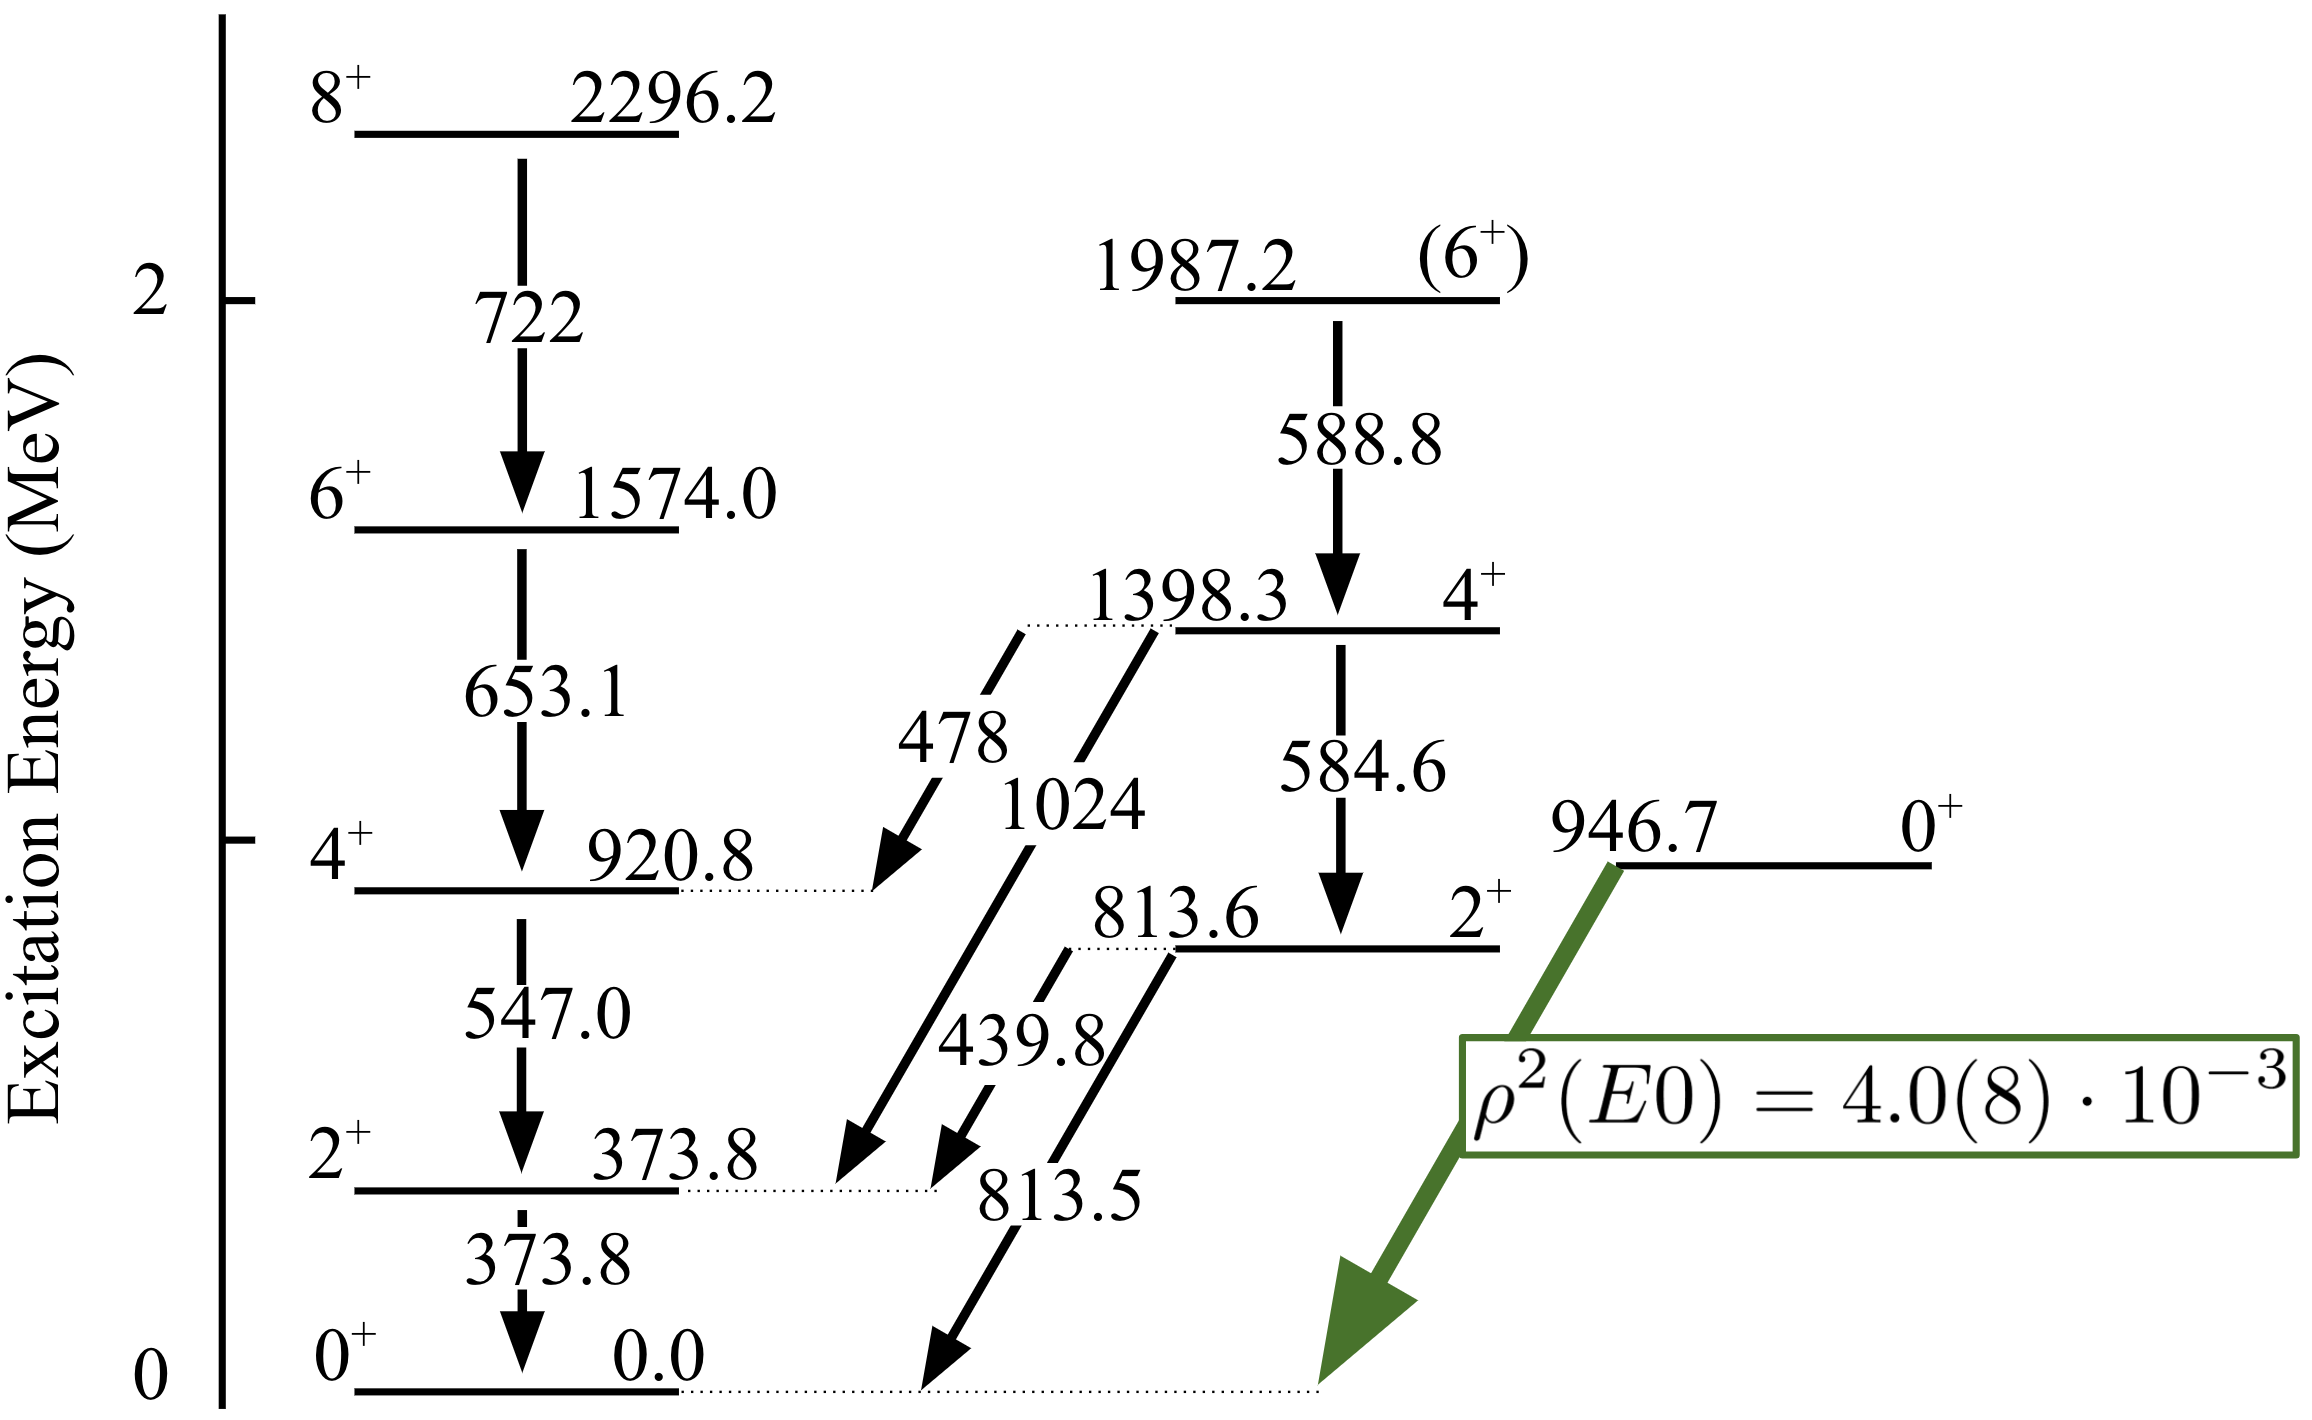
\includegraphics[width=\textwidth]{intro_110Pd_E0.png}
  \caption[Partial level scheme for the nucleus $^{110}$Pd with a previous measurement of $\rho^2(E0)$ highlighted.]{Energy levels from the first three intrinsic excitations for the nucleus $^{110}\mathrm{Pd}$ \cite{ENSDF110Pd}. State and transition energies are given in keV. The spin and parity of each state is labeled. A previous measurement of $\rho^2(E0)$ for the $0^+_2 \rightarrow 0^+_1$ transition is listed \cite{Kibedi2005}.}
  \label{figure: levels of 110Pd}
\end{figure}

This previous measurement reveals a relatively weak $E0$ transition strength for the $0_2^+ \rightarrow 0^+_1$ transition. This transition is between two intrinsic excitation bands in which the lowest energy state has a nuclear spin of 0. Different bands in a nucleus can be described by their angular momentum projection onto the axis of symmetry (the $K$ quantum number). An individual band's $K$ value is given by the nuclear spin assignment of its lowest energy level. Generally $E0$ transitions have a $\Delta K = 0$ selection rule, and the expectation was to see a low value for $\rho^2(E0)$ in the $2^+_2 \rightarrow 2^+_1$ transition \cite{CastenText}. 

In Chapter 2 the theory of the nuclear shell model, and nuclear state mixing is discussed. The modes of transition that exist for a decaying nucleus and their correspondence to nuclear properties is outlined. The experimental setup and the analysis techniques are detailed in Chapter 3. The results of the experiment are presented and discussed in Chapter 4. This work is brought to conclusion in Chapter 5, and the opportunity for potential future research is highlighted.

\endinput

Any text after an \endinput is ignored.
You could put scraps here or things in progress.

In such a transition, the dominant mode of decay is the emission of an orbital $e^-$ from the atom. This process is called internal conversion, and the electrons produced are called internal conversion electrons. Here the spatial overlap of nuclear wave functions with that of the orbital $e^-$ results in a transfer of energy to, and subsequent ejection of the $e^-$ from the atom. Given the shell structure of atomic electrons, this decay mode is most probable to occur by emission of the nearest, K shell electrons, with descending probability for shells at successively further distances from the nuclear core.

While internal conversion is the only decay mode available in these unique, zero-angular-momentum-vector-difference transitions, it is a competitive process to \gr emission in all other transitions. 
